\documentclass[12pt,letterpaper,reqno]{amsart}
\usepackage{amsmath}
\usepackage{amssymb}
\usepackage{amsthm}
\usepackage{graphicx}
\usepackage{xspace}
\usepackage[dvipsnames]{xcolor}
\usepackage{setspace}
\usepackage[letterpaper,margin=1in,headheight=15pt]{geometry}
\usepackage{bm}
\usepackage{hyperref}
\usepackage{minted}
% \definecolor{darkred}{rgb}{0.5,0.15,0.15}
% \hypersetup{colorlinks=true,urlcolor=darkred,linkcolor=darkred,citecolor=darkred}
\definecolor{hyperlinkblue}{rgb}{0,0,238}
\hypersetup{colorlinks=true,urlcolor=hyperlinkblue,linkcolor=hyperlinkblue,citecolor=hyperlinkblue}
\allowdisplaybreaks

\newtheorem{thm}{Theorem}
\newtheorem{lem}[thm]{Lemma}
\newtheorem{prop}[thm]{Proposition}
\newtheorem{cor}[thm]{Corollary}
\theoremstyle{definition}
\newtheorem{Example}[thm]{Example}
\newtheorem{Definition}[thm]{Definition}
\numberwithin{thm}{section}
\newtheorem{problem}{Problem}
\theoremstyle{remark}
\newtheorem{remark}{Remark}[section]

\usepackage{biblatex}

\addbibresource{references.bib}

\begin{document}
\onehalfspacing

\title{Math 131P Winter 2025 Final Project}
\author{George Weiksner}

\maketitle

\begin{center}
    \textbf{The Finite Difference Method}
\end{center}

\section{Introduction} \label{sec:introduction}
In Math 131p and Math 53, we learned how to solve the heat equation analytically by deriving solutions often using Separation of Variables. However, the assumption that solutions to heat equation are separable does not always hold. Specifically, when boundary conditions are more complicated. In these case and others, the heat equation may not have analytic solutions so our only option is to try solve numerically.   

Even if the heat equation can be solved analytically, we may not have enough information to solve it using an analytic solution. For example, may we are in a physical situation where we can only measure the temperature on a rod using n devices. In this case, we would not be able to generate a continuous boundary conditions for the rod. As we will see in this paper, the Finite Difference Method (FDM) gives us an opportunity to understand these problems. 

While FDM provides many benefits, it has restrictions. An important limitation to the FDM is that there must be a certain amount of data to make the solution stable. Additionally, if there is a problem has two many dimensions or too small a step size, the problem may become too complex to solve in a reasonable time/cost. Finally, the FDM applies most easy to problems with rectangular boundaries. 

The goal of this paper is to explain the Finite Difference Method which is a method to solve the heat equation numerically. First, we will derive the method. Then, we will work out a key example of using this method. I will conclude by addressing limitations to the FDM. 

\section{Solving the Heat Equation using FDM with Discrete Initial and Boundary Conditions}
\label{sec:fdm_heat}
In this section, we will learn how to solve the heat equation using the Finite Difference Method for both discrete and continuous boundary / initial conditions. The main method we will use to prove this result will be Taylor Series expansions. 

\begin{Definition}[Space and Time Grid] 
\label{def:grid}
Let the space domain $[0,L]$ be divided into $n$ equal subintervals of length

\[
h=\frac{L}{n}.
\]

Define the space grid points

\[
x_i = ih, \qquad i=0,1,\dots,n,
\]

and time grid points

\[
t_j = jk, \qquad j=0,1,2,\dots
\]

where $k$ is the time step size.
\end{Definition}

\begin{Definition}[Big-O Notation]
\label{def:bigO}
Let $f(n)$ and $g(n)$ be non-negative functions. We say that
\[
f(n) = O(g(n)) \quad \text{as } n \to \infty
\]
if there exist constants $C > 0$ and $n_0$ such that
\[
|f(n)| \le C|g(n)| \quad \text{for all } n \ge n_0.
\]

In other words, $f(n)$ grows no faster than a constant multiple of $g(n)$ for sufficiently large $n$. Colloquially, we say "$f(n)$ is upper bounded by $g(n)$."
\end{Definition}

Next, we want to find $u_xx$ to help us plug into the PDE. 

\begin{lem}
\label{lem:second_derivative}
We will show that
\[
u_{xx}(x_i,t_j) \approx \frac{u(x_{i+1},t_j)-2u(x_i,t_j)+u(x_{i-1},t_j)}{h^2}.
\]

with an error term $O(h)$. 

\begin{proof}
Using a second-order Taylor series expansions of $u(x,t_j)$ about $x_i$, we have

\[
u(x_i+h,t_j) =  u(x_i,t_j) + h u_x(x_i,t_j) + \frac{h^2}{2}u_{xx}(x_i,t_j) + O(h^3)
\]

and

\[
u(x_i-h,t_j) = u(x_i,t_j) - h u_x(x_i,t_j) + \frac{h^2}{2}u_{xx}(x_i,t_j) + O(h^3)
\]

Adding these two equations gives

\[
u(x_i+h,t_j)+u(x_i-h,t_j) = 2u(x_i,t_j) + h^2 u_{xx}(x_i,t_j) + O(h^3)
\]

Solving for $u_{xx}(x_i,t_j)$ yields

\[
u_{xx}(x_i,t_j) = \frac{u(x_i+h,t_j)-2u(x_i,t_j)+u(x_i-h,t_j)}{h^2} + O(h)
\]

Therefore, 

\[
u_{xx}(x_i,t_j) \approx \frac{u(x_i+h,t_j)-2u(x_i,t_j)+u(x_i-h,t_j)}{h^2}
\]

with an error term $O(h)$.
\end{proof}
\end{lem}

\begin{cor}
Importantly, this means that the error bound increases as $h$ increases and decreases as $h$ decreases. Since the step size $h$ is within our control, we can reduce $h$ to improve the accuracy of the approximation. However, smaller values of $h$ typically increase cost, so in practice $h$ is chosen to balance accuracy and cost.
\end{cor}

\begin{thm}
\label{thm:update_formula}
Consider the heat equation and the space and time grid introduced in Definition~\ref{def:grid}. Assume the initial temperature distribution along the rod is known, so that

\[
u(x_i,0)=a_i, \qquad i=0,1,\dots,n.
\]

This corresponds to knowing the temperature at the grid points along the rod at time $t=0$. In addition, suppose the boundary temperatures are known for all time grid points, 

\[
u(0,t_j) \quad \text{and} \quad u(L,t_j)
\]

are given for $j=0,1,2,\dots$.

Under these assumptions, we can approximate the solution $u(x_i,t_j)$ at interior grid points when the space step $h$ and time step $k$ are sufficiently small. In particular, the temperature at the next time grid point can be estimated by

\[
 u(x_i, t_{j+1}) \approx kc^2 * \frac{u(x_i+h,t_j)-2u(x_i,t_j)+u(x_i-h,t_j)}{h^2} + u(x_i, t_j)
  \]\\

\begin{proof}
From Lemma~\ref{lem:second_derivative}, we have,

\[
u_{xx}(x_i,t_j) \approx \frac{u(x_i+h,t_j)-2u(x_i,t_j)+u(x_i-h,t_j)}{h^2}.
\]

with error $O(h)$.\\

Using a one term Taylor series expansion around $x_i$ we have

\[
u(x_i,t_{j+1}) = u(x_i,t_j)+ k * u_t(x_{i},t_j) + O(k^2)\]

Solving for $u_{t}(x_i,t_j)$ yields

\[
u_t(x_{i},t_{j})  = \frac{u(x_i,t_{j+1}) - u(x_i,t_{j})}{k} + O(k)
\]\\

\[
u_t(x_{i},t_{j})  \approx \frac{u(x_i,t_{j+1}) - u(x_i,t_{j})}{k}
\]\\

with error $O(k)$.\\

Plugging both $u_{t}(x_i,t_j)$ and $u_{xx}(x_i,t_j)$ into the heat equation, we have,

\[
\frac{u(x_i,t_{j+1}) - u(x_i,t_{j})}{k} \approx c^2 *\frac{u(x_i+h,t_j)-2u(x_i,t_j)+u(x_i-h,t_j)}{h^2}
\]\\

Isolating $u(x_i,t_{j+1})$, we have,
 
 \[
u(x_i,t_{j+1})  \approx kc^2 * \frac{u(x_i+h,t_j)-2u(x_i,t_j)+u(x_i-h,t_j)}{h^2} + u(x_i,t_{j})
 \]\\

This shows that we can approximate the temperature $u(x_i, t_j)$ for small enough $h, k$ with $j \ge 0$ and $i \in {1, 2, \dots, n-1}$. This means that we can approximate points at a given time using the point to right ($u(x_{i+1},t_{j})$), the point to the left ($u(x_{i-1},t_{j})$), the current point ($u(x_{i},t_{j})$) all at the previous time step. Let's call this formula the "update formula." \end{proof}
\end{thm}

\begin{Example}
\label{ex}

Consider the heat equation solved using FDM from Theorem~\ref{thm:update_formula}

\[
u(x_i,t_{j+1})  \approx kc^2 * \frac{u(x_i+h,t_j)-2u(x_i,t_j)+u(x_i-h,t_j)}{h^2} + u(x_i,t_{j})
\]

with conditions

\[
u(0,t)=0,  u(1,t)=0, u(x,0)=[0,30,-34,47,0]
\]

and parameters $c=\frac14, L = 1, h = 0.25, k = \frac16$ and $0 \le t \le 1$\\

\textbf{Grid Setup}

Applying Definition~\ref{def:grid} with $L = 1$ and $h = 0.25$, the space grid is

\[
x=[0,0.25,0.50,0.75,1]
\]\\


Applying Definition~\ref{def:grid} with $0 \le t \le 1$ and $k = \frac16$, the time grid is

\[
t= [0, \frac16, \frac26, \frac36, \frac46, \frac56, 1]
\]\\

\textbf{Update Formula}

Now, we must find the update formula. To do this, we must first find 
\[
\frac{k c^2}{h^2}
=
\frac{\frac16 \left(\frac14\right)^2}{(0.25)^2}
=
\frac{\frac16 \cdot \frac1{16}}{\frac1{16}}
=
\frac16 .
\]

Therefore the update formula simplifies to

\[
u(x_i,t_{j+1})  \approx \frac16 * u(x_i+h,t_j)-2u(x_i,t_j)+u(x_i-h,t_j) + u(x_i,t_{j})
\]

\textbf{Algorithm}


Since the boundary values remain fixed, only the interior nodes \(x_1,x_2,x_3\) are updated. Let's compute the first iteration manually.\\

\textbf{First iteration}

For \(x_1=0.25\)

\[
u(0.25, \frac16)
\approx
\frac16(u(0.5,0)-2u(0.25,0)+u(0,0))+u(0.25,0)
\]

\[
=
\frac16(-34-2(30)+0)+30=14.3
\]

For \(x_2=0.50\)

\[
u(0.50,  \frac16)
\approx
\frac16(u(0.75,0)-2u(0.50,0)+u(0.25,0))+u(0.50,0)
\]

\[
=
\frac16(47-2(-34)+30)-34=-9.8
\]

For \(x_3=0.75\)

\[
u(0.75, \frac16)
\approx
\frac16(u(1,0)-2u(0.75,0)+u(0.50,0))+u(0.75,0)
\]

\[
=
\frac16(0-2(47)-34)+47=25.7
\]

Thus after the first time step

\[
[0,14.3,-9.8,25.7,0].
\]

Repeating the iteration yields the numerical solution

\[
\begin{array}{c|ccccc}
\label{arr}
t & x=0.00 & x=0.25 & x=0.50 & x=0.75 & x=1.00 \\ \hline
0.000000 & 0.0 & 30.0 & -34.0 & 47.0 & 0.0 \\
0.166667 & 0.0 & 14.3 & -9.8 & 25.7 & 0.0 \\
0.333333 & 0.0 & 7.9 & 0.1 & 15.5 & 0.0 \\
0.500000 & 0.0 & 5.3 & 4.0 & 10.3 & 0.0 \\
0.666667 & 0.0 & 4.2 & 5.3 & 7.6 & 0.0 \\
0.833333 & 0.0 & 3.7 & 5.5 & 5.9 & 0.0 \\
1.000000 & 0.0 & 3.4 & 5.2 & 4.8 & 0.0
\end{array}
\]
    \begin{center}
        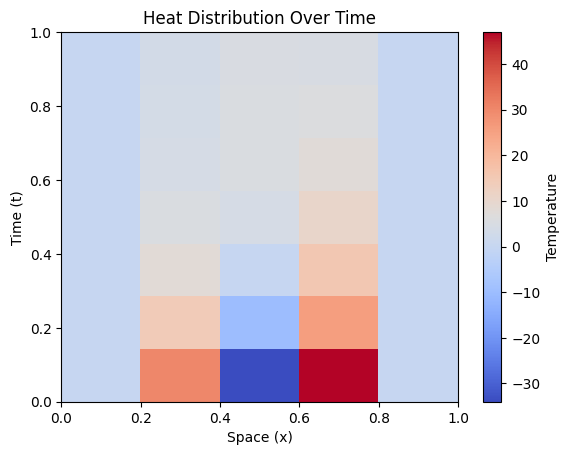
\includegraphics[width=13cm]{heat_map.png}
        \label{fig}
    \end{center}
As expected with Dirichlet boundary conditions, the solution shows that as time passes heat diffuses out the endpoints approaching 0 temperature along the rod. 
\end{Example}

\begin{prop}
Suppose the initial temperature distribution $u(x,0)=f(x)$ and the boundary temperature $u(0,t)=g(t)$ are known. Using the space and time grid from Definition~\ref{def:grid}, the heat equation can be approximated numerically using the method from Theorem~\ref{thm:update_formula}.
\end{prop}

\begin{proof}
Evaluate the initial temperature function at the space grid points:

\[
u(x_i,0)=f(x_i), \qquad i=0,1,\dots,n.
\]

Then, evaluate the boundary temperature at the time grid points:

\[
u(0,t_j)=g(t_j), \qquad j=0,1,2,\dots.
\]

These values provide the initial and boundary data required for method in Theorem~\ref{thm:update_formula}. Using

\[
u(x_i,t_{j + 1}) = + u(x_i,t_{j})+ kc^2  \frac{u(x_i+h,t_j)-2u(x_i,t_j)+u(x_i-h,t_j)}{h^2},
\]

we can compute approximate temperatures at interior grid points for
$j\ge0$ and $i=1,\dots,n-1$.
\end{proof}

\section{Additional Limitations of the Finite Difference Method}
\label{sec:limitations}

While FDM is a powerful method for approximating solutions to PDEs, stability requirements and computational complexity limit its applicability. 

\begin{Definition}[Stability Condition]
\label{def:stability}
For the solution for the heat equation to remain stable, the following relation must be satisfied: 

\[
\frac{c^2 k}{h^2} \le \frac{1}{2}.
\]

If this condition is not satisfied, then numerical errors may grow exponentially with each time step.\\
\end{Definition}

\begin{cor}
Importantly, note that this coefficient is proportional with $k$, the step size for time, and inversely proportional for $h^2$. The constant $c$ is out of your control because it is a constant related to nature. What this means if you are solving a practical problem is that if you want higher time granularity in your measurements, it is going to cost you stability and you may have to increase the number of sensors you use initially on your rod (increase space granularity).  

Remember that $c$ and $h$ also have to be small enough for the Taylor series approximations to be within an acceptable range of accuracy. 
\end{cor}

\begin{thm}[Computational Complexity]
\label{thm:complexity}
Let a space domain be divided into $n$ grid points and the time interval be divided into $m$ steps. The finite difference method requires approximately $O(nm)$ computations.
\end{thm}

\begin{proof}
At each time step $t_j$, the method computes values at the interior grid points $i=1,\dots,n-1$. Thus each time step requires roughly $n$  operations. Repeating this process for $m$ time steps yields approximately $nm$ total computations.
\end{proof}

In practical problems, you may only have a certain amount of compute you can deploy to a specific problem. This constraint alongside the stability condition can usability and accuracy of FDM. Additionally, the nature of experiment / physical situation may add another constraint. 

\section{Conclusion}
In this paper, the correctness of the Finite Difference Method was proven for the heat equation using a Taylor Series expansion, an example problem of this method was shown, and limitations were discussed (specifically computational complexity, stability, Taylor Series convergence).

This paper leaves more room for exploration. More specifically, the process of solving higher dimensional heat equations and other PDEs using the Finite Difference Method. Another area of further research is considering a more rigorous treatment to the stability condition. 

As a math major with interested in how theoretical understandings can impact applied settings, learning how to solve PDEs numerically is a great opportunity. I was able to see the power of solving applied math problems but also the limitations that need to be considered when solving a practical problem. More specifically, I was fascinated by the trade offs between stability, cost, and the convergence of the Taylor Series. I am excited in my math / computer science journey going forward to consider applying a theoretical understanding of a concept to better solve applied problems.  


\printbibliography

% Below are appendices sections (if needed)

\appendix

\section{Data Tables}

This appendix contains the data inputed and produced by the finite difference method described in Example~\ref{ex}. The tables below list the initial conditions, boundary conditions, and solution grid.

\subsection{Simulation Parameters}

\begin{center}
\begin{tabular}{|c|c|}
\hline
Parameter & Value \\
\hline
Rod length $L$ & 1 \\
Space step $h$ & 0.25 \\
Time step $k$ & $\frac{1}{6}$ \\
Diffusion constant $c$ & $\frac{1}{4}$ \\
Number of spatial nodes & 5 \\
Number of time steps & 7 \\
\hline
\end{tabular}
\end{center}

\subsection{Initial Temperature Distribution}

\begin{center}
\begin{tabular}{|c|c|}
\hline
$x$ & $u(x,0)$ \\
\hline
0.00 & 0 \\
0.25 & 30 \\
0.50 & -34 \\
0.75 & 47 \\
1.00 & 0 \\
\hline
\end{tabular}
\end{center}

\subsection{Boundary Conditions}

\begin{center}
\begin{tabular}{|c|c|c|}
\hline
$t$ & $u(0,t)$ & $u(1,t)$ \\
\hline
0.000000 & 0 & 0 \\
0.166667 & 0 & 0 \\
0.333333 & 0 & 0 \\
0.500000 & 0 & 0 \\
0.666667 & 0 & 0 \\
0.833333 & 0 & 0 \\
1.000000 & 0 & 0 \\
\hline
\end{tabular}
\end{center}

\subsection{Numerical Solution Grid}

The following table shows the approximate solution $u(x_i,t_j)$ computed using the update formula derived in Theorem~\ref{thm:update_formula}.

\begin{center}
\begin{tabular}{|c|c|c|c|c|c|}
\hline
$t$ & $x=0.00$ & $x=0.25$ & $x=0.50$ & $x=0.75$ & $x=1.00$ \\
\hline
0.000000 & 0.0 & 30.0 & -34.0 & 47.0 & 0.0 \\
0.166667 & 0.0 & 14.3 & -9.8 & 25.7 & 0.0 \\
0.333333 & 0.0 & 7.9 & 0.1 & 15.5 & 0.0 \\
0.500000 & 0.0 & 5.3 & 4.0 & 10.3 & 0.0 \\
0.666667 & 0.0 & 4.2 & 5.3 & 7.6 & 0.0 \\
0.833333 & 0.0 & 3.7 & 5.5 & 5.9 & 0.0 \\
1.000000 & 0.0 & 3.4 & 5.2 & 4.8 & 0.0 \\
\hline
\end{tabular}
\end{center}


\section{Codes}
Here are the codes used to generate the results presented in this paper. \\

\subsection{Finite Difference Method Function}
The implementation was used to produce the array shown in Array~\ref{arr}. This function was used to solve a 1D problem using the Finite Difference Method. \\


\begin{minted}{python}
def heat_fdm(initial, left_bc, right_bc, L=1, T=1, c=1):
    """ 
    Finite difference solver for the heat equation.

    initial : list
        values of u(x_i,0)

    left_bc : list
        boundary values at x=0 for each time step

    right_bc : list
        boundary values at x=L for each time step
    
    L = length of rod

    T = time to solve for

    c = diffusion constant
    """

    n = len(initial) - 1
    m = len(left_bc) - 1

    h = L / n
    k = T / m

    s = c**2 * k / h**2

    # solution array
    u = np.zeros((m+1, n+1))

    # initial condition
    u[0, :] = initial

    # boundary conditions
    for j in range(m+1):
        u[j, 0] = left_bc[j]
        u[j, -1] = right_bc[j]

    # finite difference iteration
    for j in range(m):
        for i in range(1, n):
            u[j+1, i] = u[j, i] + s * (u[j, i+1] - 2*u[j, i] + u[j, i-1])
            
    x = np.linspace(0, L, n+1)
    t = np.linspace(0, T, m+1)
    grid = pd.DataFrame(u, columns=[f"x{i:.2f}" for i in x])
    grid = grid.round(1)
    grid.insert(0, "t", t)


    return grid
\end{minted}

\subsection{Heatmap Function}
This function was used to generate the heatmap in Figure~\ref{fig}.\\

\begin{minted}{python}
def heatmap(grid): 
    t = grid["t"].values
    x = np.array([float(col[1:]) for col in grid.columns if col != "t"])
    heat = grid.drop(columns="t").values

    plt.imshow(
        heat,
        aspect='auto',
        origin='lower',
        extent=[x.min(), x.max(), t.min(), t.max()],
        cmap='coolwarm'
    )

    plt.xlabel("Space (x)")
    plt.ylabel("Time (t)")
    plt.title("Heat Distribution Over Time")

    plt.colorbar(label="Temperature")
    plt.show()
\end{minted}

\subsection{Main}
This code was ran after the first two functions to produce the results themselves.\\

\begin{minted}{python}
initial = [0, 30, -34, 47, 0]
left_bc = [0, 0, 0, 0, 0, 0, 0]
right_bc = [0, 0, 0, 0, 0, 0, 0]

print("Inital Condition:", initial)
grid = heat_fdm(initial, left_bc, right_bc, c = 1/4)

print(grid)
heatmap(grid)
\end{minted}

\end{document}